\chapter{HDF5 C++ Interface}
%\section{Example Section}
%\subsection{Example Subsection}
%\subsubsection{Example Subsubsection}
%\paragraph{Example Paragraph}
%\subparagraph{Example Subparagraph}
\section{Overview}
The acronym HDF stands for hierarchical data format meaning this binary format is allowing to structure the internal objects after the users demand. This structure is quite similar to a file system where data is ordered with folders and sub-folders. For more detailed information see the official C \cite{hdf5cdoc} and C++ \cite{hdf5cppdoc} documentation. The reason why also the C documentation is very important is based on the fact that the C++ implementation is mostly a nice wrapper based on the C implementation. For the exact dependence see table \ref{table:corrs}.
\begin{figure}[ht!]
\centering
\begin{tabular}{|l|l|}
\hline
HDF5 C APIs&C++ Classes\\
\hline
Attribute Interface (H5A)&Attribute\\
Datasets Interface (H5D)&DataSet\\
Error Interface (H5E)&Exception\\
File Interface (H5F)&H5File\\
Group Interface(H5G)&Group\\
Identifier Interface (H5I)&IdComponent\\
Property List Interface (H5P)&PropList and subclasses\\
Dataspace Interface (H5S)&DataSpace\\
Datatype Interface (H5T)&DataType and subclasses\\
\hline
\end{tabular}
\caption{Table of correspondence between C and C++}
\label{table:corrs}
\end{figure}
To use the C++ language features to its most capabilities inheritance is used. This allows reuse of functions, objects and properties over many hierarchy layers. This enforces a strict dependence when sharing or creating objects. To have an overview on the hierarchy look at figure \ref{graph:hierarchy}.

\begin{figure}[ht!]
\centering
\resizebox{\textwidth}{!}{
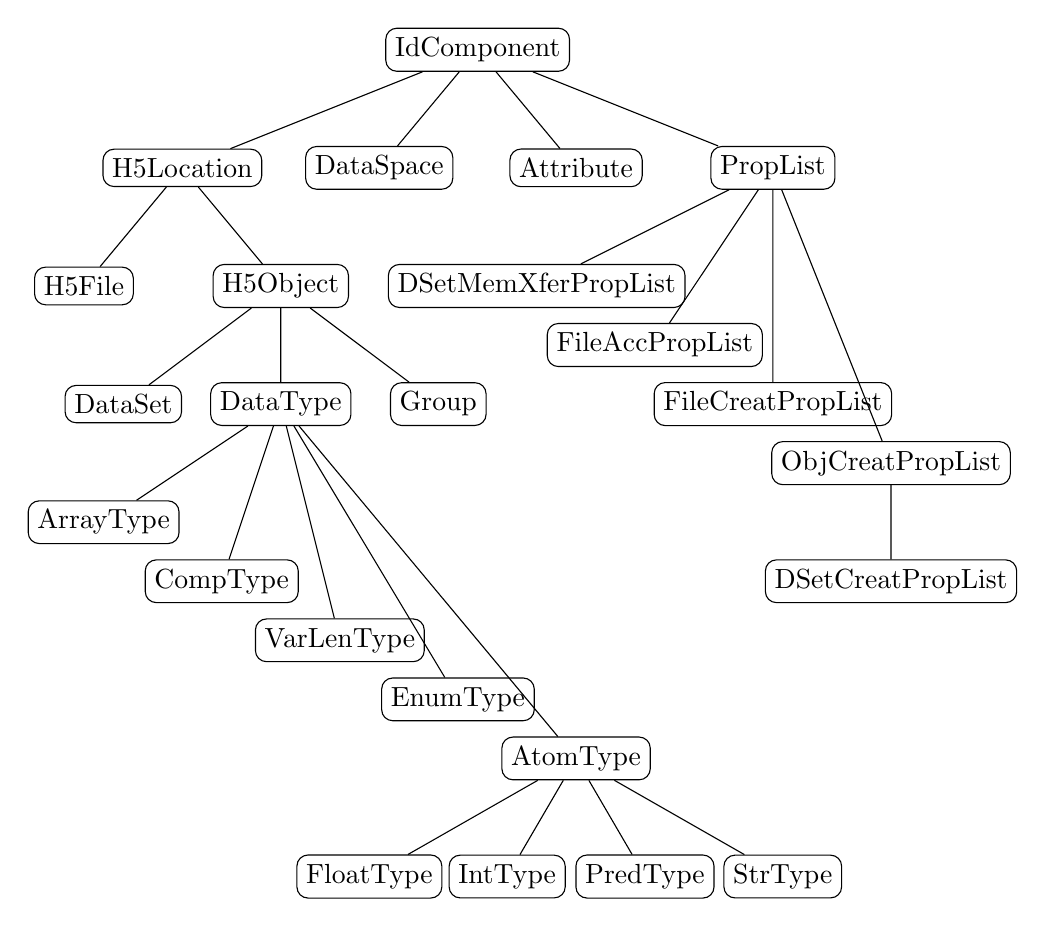
\begin{tikzpicture}[
baseline,
every node/.style = {shape=rectangle, rounded corners, draw, align=center},
]]
  \node {IdComponent}
    child[xshift=-1.5cm]
    {
        node{H5Location}
    	child[xshift=-0.5cm]{node{H5File}}
    	child[xshift=0.5cm]
    		{
    		node{H5Object}
    		child[xshift=-0.5cm]{node{DataSet}}
    		child{
    			node{DataType}
    			child[xshift=0.75cm]{node{ArrayType}}
    			child[xshift=0.75cm,yshift=-0.75cm]{node{CompType}}
    			child[xshift=0.75cm,yshift=-1.5cm]{node{VarLenType}}
    			child[xshift=0.75cm,yshift=-2.25cm]{node{EnumType}}
    			child[xshift=0.75cm,yshift=-3.0cm]
    				{
    				node{AtomType}
    				child[xshift=-0.375cm]{node{FloatType}}
    				child[xshift=-0.125cm]{node{IntType}}
    				child[xshift=0.125cm]{node{PredType}}
    				child[xshift=0.375cm]{node{StrType}} 
    				}
    			}
    		child[xshift=0.5cm]{node{Group}}
    		}
 	}
    child[xshift=-0.5cm]{node{DataSpace}}
    child[xshift=0.5cm]{node{Attribute}}
    child[xshift=1.5cm]{
    	node{PropList}
    	child[xshift=-0.75cm]{node{DSetMemXferPropList}}
    	child[xshift=-0.75cm,yshift=-0.75cm]{node{FileAccPropList}}
    	child[xshift=-0.75cm,yshift=-1.5cm]{node{FileCreatPropList}}
    	child[xshift=-0.75cm,yshift=-2.25cm]{
    		node{ObjCreatPropList}
    		child{node{DSetCreatPropList}}
    		}
    		};
\end{tikzpicture}
}
\caption{Depiction of derivation hierarchy}
\label{graph:hierarchy}
\end{figure}

As stated in the background this project is about the simulation of \textit{Hagedorn} wavepackets over a fixed time horizon. To keep track and possibly reproduce the results the wavepackets have to be saved in every time step $\Delta t$ of the simulation. This has to be achieved with the classes shown in figure \ref{graph:hierarchy}. To understand the functionality of these classes they will be explained in the following sections.

\section{Internal types and states}
An interface in general has supported objects and functions. These functions also have preconditions and postconditions whereas objects have valid states. In case of the HDF5 library when these are not fulfilled an exception is thrown which could abort or interrupt the program execution. Therefore it is important to always use valid objects and function calls. There are two noteworthy types which are also used the most. These are \texttt{hsize\_t} and \texttt{H5std\_string}. Variable of type \texttt{hsize\_t} represent native multiple-precision integer. This type substitutes the C++ internal \texttt{int} data type. The \texttt{H5std\_string} type is just an alias for the \texttt{std::string} data type from the standard library. Internal valid states are represented in only uppercase letters and with the C prefix as in table \ref{table:corrs}. For example a valid property list state is \texttt{H5P\_DEFAULT}.

\section{H5File}
As the name already suggest this class is used to manage the binary file object. When a \textit{H5File} is default constructed it also allocates a default \textit{Group} root named "/". To construct a \textit{H5File} a minimal number of two arguments is needed. The two additional optional arguments are a \textit{FileCreatPropList} and a \textit{FileAccPropList} which would allow further specification. These would be creation and access properties as suggested by the names. In case of this project they are not needed and the \texttt{H5P\_DEFAULT} is sufficient. For the first mandatory argument, which is the filename, a \texttt{H5std\_string} or as discussed before a string required. The second mandatory argument defines the type of creation which at default has two valid values. These possible values are \textit{H5F\_ACC\_TRUNC} and \textit{H5F\_ACC\_EXCL} which are mutually exclusive. The former truncates the file meaning if it already exists erase all data previously stored in the file. The latter fails if the file already exists under the specified name which ends in an exception. It is advised to work with \textit{H5F\_ACC\_TRUNC} because it is simpler and thus errors will less frequently occur.

\section{Group}
As previously mentioned it is a hierarchical data format. The hierarchy gets implement through the usage of \textit{Groups}. In case of a \textit{Hagedorn} wavepackets and its corresponding energies the structure in figure \ref{graph:file} is preferred as it corresponds to the structure of the python implementation.

\begin{figure}[ht!]
\centering
\resizebox{\textwidth}{!}{
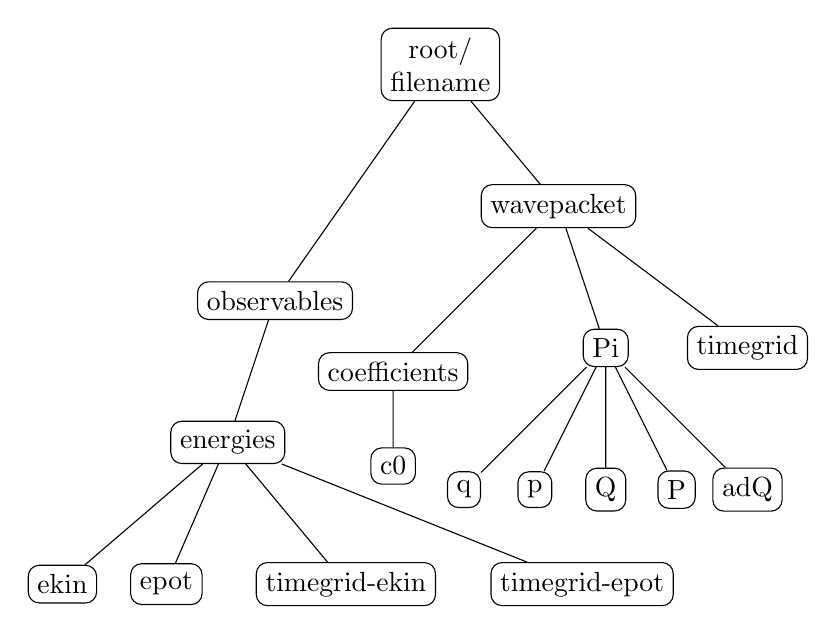
\begin{tikzpicture}[
baseline,
scale=1.2,
every node/.style = {shape=rectangle, rounded corners, draw, align=center},
]]
  \node {root/\\filename}
    child[yshift=-1cm,xshift=-1cm]
    {
    node{observables}
    child[xshift=-0.5cm]
            {
            node{energies}
    		child[xshift=0.5cm]{node{ekin}} 
    		child[xshift=0.1cm]{node{epot}}
    		child[xshift=0.5cm]{node{timegrid-ekin}}
    		child[xshift=1.5cm]{node{timegrid-epot}}
    		} 
    }
    child[xshift=0.5cm] 
    { 
    node {wavepacket}
    child[xshift=-0.25cm,yshift=-0.25cm]{node{coefficients}
    child[yshift=0.5cm]{node{c0}}}
    child[xshift=0.5cm]
    {
    node {Pi}
    child[xshift=1.5cm]{ node {q} }
    child[xshift=0.75cm] { node {p} }
    child { node {Q} }
    child[xshift=-0.75cm] { node {P} }
    child[xshift=-1.5cm] { node {adQ}}    
    }
    child[xshift=0.5cm]{node{timegrid}} 
	};
\end{tikzpicture}
}
\caption{Depiction of desired internal structure of a H5File}
\label{graph:file}
\end{figure}
To create a \textit{Group} only a \texttt{string} argument is required which acts as name but more importantly also as path similar to figure \ref{graph:file}. As previously indicated a \textit{H5File} has root \textit{Group} "/" by default after allocation. To accomplish the structure as in figure \ref{graph:file} the path is included in the name. For instance to have a \textit{Group} "wavepacket" after the root "/" and a \textit{Group} "Pi" after "wavepacket" the first name will be modified to "/wavepacket" and the second to "/wavepacket/Pi". This implies that every intermediate node in figure \ref{graph:file} will be a \textit{Group}. The leafs however will be \textit{DataSets} which will be explained in the next section.

\section{DataSet}
\section{DataType}
The language C++ itself supports data types such as int, double, char etc. but these cannot be used directly in a binary data format. The reason for this 
\section{DataSpace}
\section{PropList}
\subsection{DSetCreatePropList}
\section{Attribute}



\chapter{Writer Template}

\section{DataType Declaration}

\section{Setup write options}

\section{Setup write hierarchy}

\section{Prestructure}

\section{Selection}

\section{Transformation}

\section{Writing}

\section{Extension}

\section{Update}

\section{Poststructure}

\section{Inner workings in a picture}

\section{Usage in a simulation main file}


\chapter{Data Test}

\section{Introduction to GoogleTest}

\section{The Main C++ File}


\chapter{Conclusion}

